\chapter{Overzicht van de technologie}
\todo{Inleiding}
\section{Geschiedenis van de databasemanagementsystemen}
Doorheen de geschiedenis, heeft de mens verschillende manieren gebruikt om data op te slaan en nadien terug te vinden. Doorheen de geschiedenis zijn er verschillende stappen van data management geweest, tot voor het ontstaan van de computer ging dit met pen en papier of met ponskaarten\cite{gray2007data}. Met de opkomst van de computer, werden nieuwe methodes gebruikt die doorheen de tijd zijn mee geëvolueerd met de vooruitgang in de technologie en de veranderingen in het gebruik van de data. De hiervoor ontwikkelde software wordt gecategoriseerd onder het \textbf{databasemanagementsysteem}(\glspl{DBMS}). De ontwikkeling en opkomst van de \glspl{DBMS} kan in verschillende fasen opgedeeld worden.  

De eerste \glspl{DBMS} zijn er gekomen met de introductie van de mainframes zoals UNIVAC1 en de ontwikkeling van specifieke programmeertalen voor het werken met deze data, onder andere conferenties zoals CODASYL hebben de ontwikkeling van COBOL en andere standaarden mee ontwikkeld\cite{gray2007data}. \todo{Mss ook het toevoegen van IBM hier + (IDS)?}   

De volgende grote verandering in \glspl{DBMS} is er gekomen door het artikel van E. Codd over het relationele model in 1969 \cite{codd1970relational}. De sleutel concepten van het relationele model is dat de data georganiseerd is in relaties (tabellen) die gekoppeld zijn door middel van keys (constraints) waarbij redundante data wordt vermeden. 
Voorbeelden van populaire \glspl{DBMS} (relationele \glspl{DBMS}) die het model implementeren zijn Oracle, MySQL en PostgreSQL. Meer informatie komt aanbod in de volgende sectie. 

De laatste nieuwe generatie zijn NoSQL databases die sinds 2000 zijn begonnen, NoSQL staat voor '\textit{Not only SQL}'. Deze systemen zijn er gekomen als reactie op het relationele model voor een meer flexibele database, lagere complexiteit, hogere doorvoer van data, horizontale schaalbaarheid en het draaien op commodity hardware.  Verschillende voorbeelden van NoSQL systemen zijn Google BigTable, Amazon Dynamo, HBase, MongoDB, ... \cite{Strauch.NoSQL} Meer informatie en een vergelijking met relationele databases komt aanbod in de volgende sectie. 

\section{Relationele en NoSQL databases} 
\todo{Yeaah}
\subsection{Relationele database}
Een R\gls{DBMS} is een \gls{DBMS} gebaseerd op relationele model voor het structuren van de database.

Het relationele model is gebaseerd op theoretische wiskundige principes zoals de set-theorie en eerste-orde predicaten logica. Het model organiseert de data in tabellen en relaties tussen de relaties. De tabel heeft kolommen die verschillende velden voorstellen en elke rij een collectie van gerelateerde datawaardes is. De relaties tussen de verschillende tabellen toont mogelijke connecties. Een belangrijke eigenschap is dat de tabellen en relaties genormaliseerd worden, hiermee wordt redundante informatie verwijderd. Dit zorgt voor een hogere data integriteit en een vermindering in data anomalieën die kunnen optreden bij een update.\cite{Elmasri:2010:FDS:1855347} \\
Dit kan geïllustreerd worden met het korte voorbeeld in figuur \ref{fig:Relationeel-Model-Normalisatie}: de professor voor een vak zal bij elke student hetzelfde zijn, het veranderen van een professor voor een vak zou in het eerste geval een update van alle ingeschreven studenten inhouden, in het tweede geval is dit maar één enkel record, hetzelfde geldt voor de student. \\
Interactie met de R\gls{DBMS} gebeurt op basis van SQL (Structured Query Language), een taal gebaseerd op de relationele logica geeft uitgebreide query mogelijkheden aan de gebruiker van de software.   
\begin{figure}[h!]
\centering
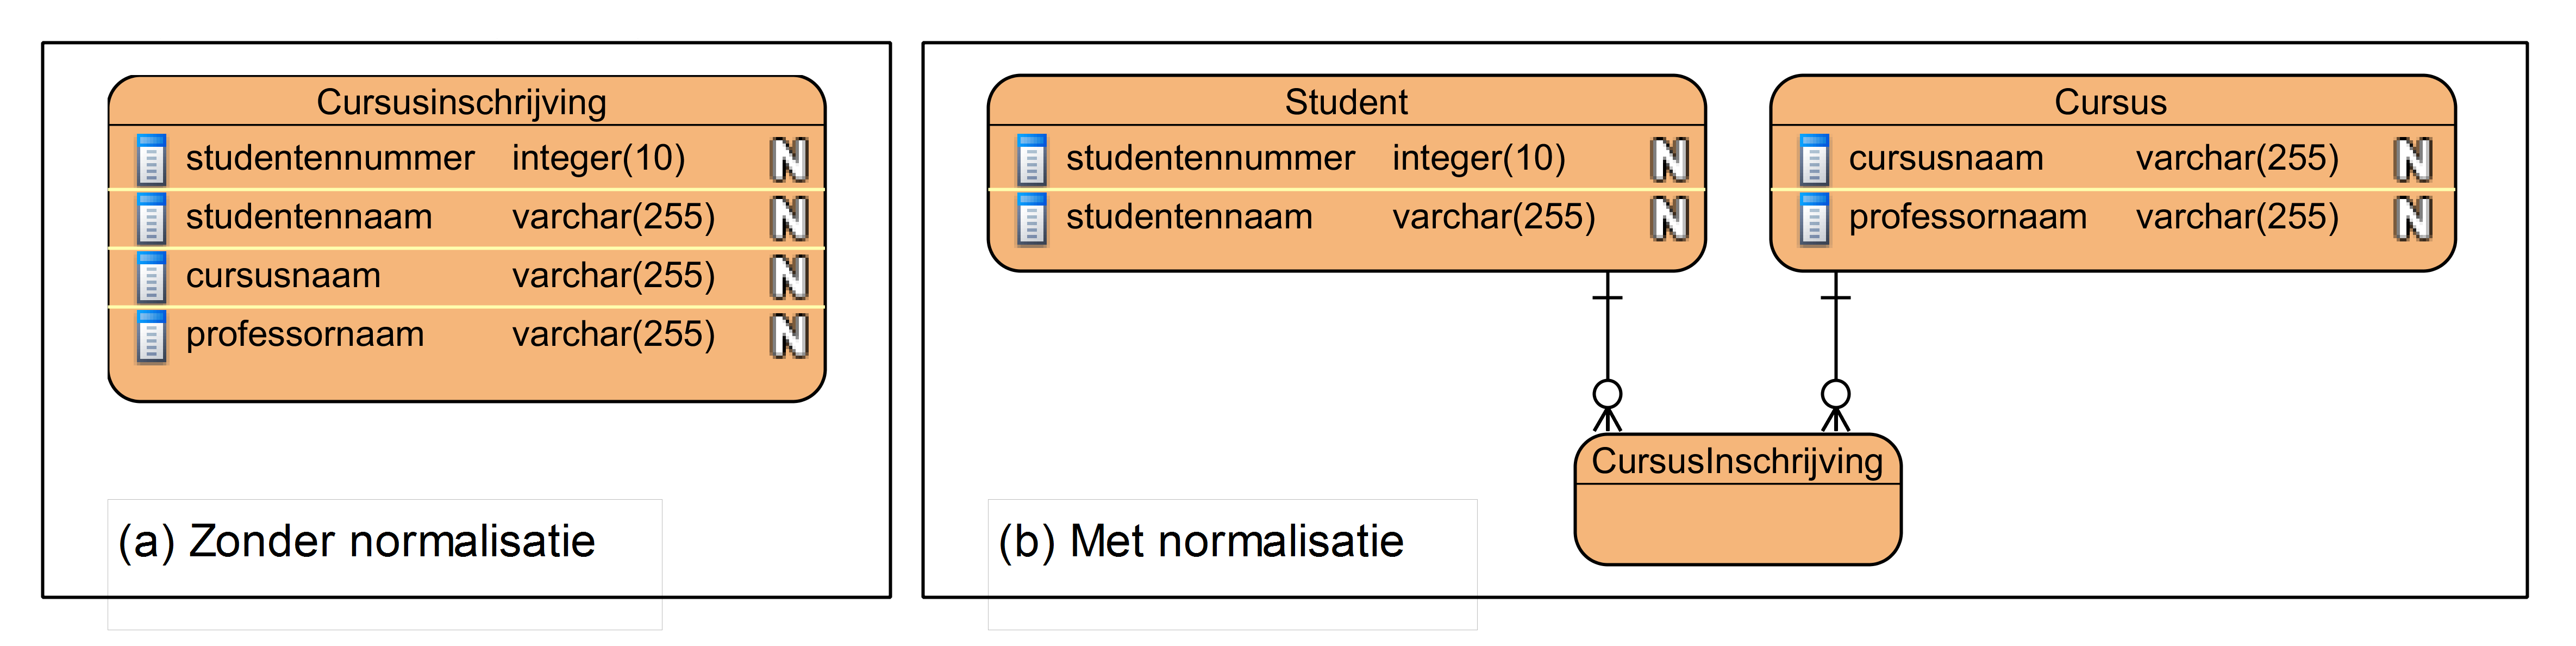
\includegraphics[width=\linewidth]{img/Relationeel-Model-Normalisatie.png}
\caption[Relationeel datamodel (a) zonder en (b) met normalisatie]{Relationeel datamodel (a) zonder en (b) met normalisatie}
\label{fig:Relationeel-Model-Normalisatie}
\end{figure}

Een belangrijk concept in een relationele database is ACID tussen verschillende transacties:

\paragraph{Atomair (\underline{A}tomicity)} Een database transactie moet oftewel volledig uitgevoerd worden oftewel heeft geen enkele databasebewerking plaatsgevonden. 

	\paragraph{Consistent (\underline{C}onsistency)} Een transactie behoudt de consistentie als de volledige uitvoering van de transactie de database van één consistente staat naar een andere brengt. Een consistente staat is een staat die ervoor zorgt dat waardes van een instantie consistent zijn met de andere waarden in dezelfde staat. Een voorbeeld is het overschrijven van \euro{50} van persoon A naar B, op het einde moet de totale som nog steeds gelijk zijn, A \euro{50} minder en B \euro{50} meer. 
	
	\paragraph{Geïsoleerd (\underline{I}solation)} Een transactie moet uitgevoerd worden alsof ze geïsoleerd is van andere transacties, die eventueel gelijktijdig uitgevoerd worden. 
	
	\paragraph{Duurzaam (\underline{D}urability)} Een voltooide transactie kan later niet ongedaan gemaakt worden.
Deze verschillende concepten bieden de gebruiker van het R\gls{DBMS} garanties die de programmeur van de database kan gebruiken voor zijn systeem. Daartegen over staat wel dat dit de complexiteit van de RDBMS groeit, ook indien dit voor bepaalde toepassingen misschien niet nodig is.

\subsection{NoSQL database}\label{sec:eventualconsistency}
NoSQL DBMS zijn ontstaan als reactie op 'one size fits all'-gedachte die R\glspl{DBMS} volgen. Dit is ook zichtbaar in de verschillende NoSQL systemen, ze bestaan in verschillende variëteiten, elk voor met hun eigen eigenschappen en toepassingsgebied, toch is er een rode draad te vinden tussen de verschillende systemen vergeleken met R\gls{DBMS}: 
\begin{itemize}
	\item \textbf{Lagere complexiteit}: NoSQL systemen bieden minder opties en features aan dan de R\gls{DBMS} omdat veel applicaties die nu eenmaal niet nodig hebben. Bijvoorbeeld in een sociale netwerk moet een post niet onmiddellijk beschikbaar zijn voor al de vrienden van een persoon, maar dit mag even duren.
	\item \textbf{Hogere doorvoer}: Talrijke NoSQL systemen bieden een hogere doorvoer van data aan, meestal gecombineerd met een lagere complexiteit. 
	\item \textbf{Horizontale schaalbaarheid en werkend op commodity hardware}: Waar grote R\glspl{DBMS} draaien op dure high-end systemen, was het bedoeling van NoSQL databases om te werken met eenvoudige machines (commodity hardware). \\
	Horizontale schaalbaarheid staat voor het toevoegen extra machines aan een systeem voor extra resources, in tegenstelling tot verticale schaalbaarheid waar krachtigere machines worden gebruikt. In horizontale opschaling wordt de data van een enkele database verspreid over verschillende machines die elk maar een deel opslaan.\\
	NoSQL systemen combineert deze twee elementen en biedt hierdoor een schaalbaar systeem aan met basis componenten.
	\item \textbf{Datamodel dichter bij objecten}: De meeste NoSQL systemen zijn zodanig ontworpen dat deze de vertaling van objecten naar opslag eenvoudiger of meer gelijkend maken dan R\glspl{DBMS}.  
\end{itemize}  \noindent
Deze verschillende argumenten, leiden vervolgens tot een tegenreactie op ACID: BASE. \noindent
\begin{itemize}
 \item Basis beschikbaarheid (\textbf{B}asically \textbf{Availability}): Een applicatie werkt zo goed als heel de tijd.
 \item \textbf{S}oft State: De data moet op een bepaald moment niet volledig consistent zijn. 
 \item Eventuele consistentie (\textbf{E}ventual Consistency): De database zal na enige tijd in een consistente status uitkomen. Eventuele consistentie kan op zijn beurt opnieuw onderverdeeld worden in 4 categorieën \cite[slide 16]{lipcon2009design}:  \todo{Ga hier dieper op in}
 	\begin{itemize}
 		\item \textit{Read your own writes} consistentie: Ongeachte van de server waarop een gebruiker leest, zal hij zijn update onmiddellijk correct lezen. 
 		\item \textit{Session} consistentie: De gebruiker zal zijn updates onmiddellijk kunnen lezen binnen dezelfde sessie, een sessie is hierdoor meestal gelimiteerd tot een enkele databaseserver. 
 		\item \textit{Casual} consistentie: Als een gebruiker versie X leest en vervolgens versie Y schrijft, zal elke gebruiker die versie Y leest ook versie X lezen.
 		\item \textit{Monotonic Read} consistentie: Dit levert monotone tijdsgaranties dat een gebruiker enkel recentere data versies in de toekomst zal lezen. 
 	\end{itemize}
\end{itemize}

\subsubsection{Classificatie van NoSQL systemen}
Er zijn vele NoSQL systemen ontworpen gedurende de laatste jaren, elk met hun eigen variëteit en functionaliteit. Er bestaan verschillende manieren om de systemen te classificeren, maar één van de meest gebruikte doet dit op basis de data modelering, een korte vergelijking bevindt zich in tabel \ref{table:selectie-classificatie}.  

\begin{table}[!h]
	\resizebox{\textwidth}{!} {
		\begin{tabular}{l l l l l l l}
			\textbf{Soort} & \textbf{Performantie} & \textbf{Schaalbaarheid} & 			\textbf{Flexibiliteit} & \textbf{Complexiteit} & \textbf{Functionaliteit} \\ \hline
			Column & hoog & hoog & gematigd & laag & minimaal \\
			Document & hoog & variabel(hoog) & hoog & laag & variabel (laag) \\
			Graph & variabel & variabel & hoog & hoog & graph theory \\
			Key-Value & hoog & hoog & hoog & geen & variabel (geen) \\
		\end{tabular}
	}
	\caption{Classificatie en categorisatie van NoSQL \glspl{DBMS} door Scofield en Popescu. \cite{categorizatie-sco10} \cite{categorizatie-pop10b} }
	\label{table:selectie-classificatie}
\end{table} 

\paragraph{Column Model}In een column-gebaseerd systeem wordt de data opgeslagen per kolom in plaats van de traditionele manier, per rij. Deze aanpak werd in eerste instantie gedaan voor analyse van business intelligentie. Het systeem is geïnspireerd door de paper van Google’s Bigtable \cite{chang2008bigtable}. \cite{Strauch.NoSQL}

\paragraph{Graph Model} In een grafen model, wordt de data voorgesteld en opslagen volgens de grafen theorie: knopen, lijnen en eigenschappen op de knopen en lijnen. \cite{bollacker2008freebase}.   

\paragraph{Document Model} Document systemen zijn volgens vele de volgende stap in key-value systemen, waar deze complexere structuren toe laten, dit door middel van meerdere key/value paren per element. \cite{Strauch.NoSQL} \\
Een document moet geen vaste structuur hebben maar elk document op zich kan verschillende velden hebben, dit kan bijvoorbeeld gezien worden bij boeken. Waar een bepaald boek een recept is, kan een ander een deel zijn van een trilogie. Bij het eerste kan de kooktijd bijvoorbeeld apart opgeslagen worden en bij de tweede de andere boeken. 

\paragraph{Key/Value Model} Key-value systemen hebben een heel eenvoudig data model, data kan opgeslagen, opgevraagd en verwijderd worden op basis van een key. De informatie die in de database zit, is de waarde voor die key. \\
Met dit eenvoudig model en functionaliteit die weinig complexiteit introduceren, kan er gestreefd worden naar een hoge performantie, schaalbaarheid en flexibiliteit. \cite{Strauch.NoSQL}

\todo{extra conclusion text?}
\section{Bespreking van verschillende \glspl{DBMS}}\label{sec:BesprekingDBMS}
De verschillende categorieën databases zijn besproken, voor deze thesis zullen enkele relationele en NoSQL \glspl{DBMS} in meer detail worden besproken. Databases uit de volgende 4 categorieën komen verder aanbod, er is gekozen om de Graph NoSQL \glspl{DBMS} niet te bespreken omdat deze een heel andere dataset ondersteunen als de overige categorieën. 
\begin{itemize}
\item Column NoSQL \glspl{DBMS}: Cassandra, HBase
\item Document NoSQL \glspl{DBMS}: Apache CoucheDB, MongoDB
\item Key-Value NoSQL \glspl{DBMS}: LightCloud (Tokyo), MemCache, Redis, Riak, Project Voldemort
\item Relationele NoSQL \glspl{DBMS}: MySQL, Pgpool-II (PostgreSQL)
\end{itemize}

\subsection{Column database}\todo{Nalezen}
\subsubsection{Cassandra}
\textit{Website: \url{http://cassandra.apache.org/}}\\
Cassandra is een database die gebaseerd is op 2 verschillende systemen, Amazon's Dynamo en Google's Bigtable, wat voor een combinatie van een column- en key-value-based database zorgt. 

De query taal is beperkt tot 3 operaties: get, insert en delete \cite{Lakshman:2010:CDS:1773912.1773922}, waar de  laatste waarde in geval van een conflict zal opgeslagen worden.

De database kan gedistribueerd uitgerold worden waar door middel van partitionering en een consistent hashing algoritme de data verspreid wordt over de verschillende instanties. Om beschikbaarheid van de data te hebben bij een failure, wordt deze gerepliceerd over verschillende instanties met verschillende configuratie modellen. 

\subsubsection{HBase}
\textit{Website: \url{http://hbase.apache.org/}}\\
HBase is een database die gebaseerd is op Google's BigTable en draait boven op HDFS, Hadoop Distibuted File System.

De query taal voor HBase bestaat uit 4 elementen, een get, put en delete als standaard operaties en een scan om over verschillende rijen te gaan. 

Voor het gedistribueerd draaien van de database, wordt de database ingedeeld in regio's. Vervolgens is een verantwoordelijk voor regio's  Regionserver om de data van regio's op te slaan. Daarnaast is er ook nog afhankelijkheid van Zookeeper voor management van regio's en name en data-instanties als opslag.  

\subsection{Document database}
\subsubsection{Apache CoucheDB}
\textit{Website: \url{http://couchdb.apache.org/}}\\
Apache CoucheDB is een document database waar alles wordt voorgesteld met behulp van JSON. De database kan bevraagd worden door middel van Map-Reduce, de map gebeurd door een \textit{view}, een JavaScript-functie die de gegevens zal selecteren. Nadien kan met een reduce view de data geaggregeerd worden. 

Bij het gedistribueerd uitrollen zal de data met consistent hashing over verschillende instanties verdeeld worden waar elke instantie een zelfde rol heeft. Nu zal CoucheDB enkel updates van data van instantie veranderen en niet data automatisch load-balancen. Ook is het mogelijk om een exacte replica van de ene naar de andere instantie te sturen, dit wordt bijvoorbeeld handig indien documenten naar een laptop gesynchroniseerd worden om later offline te kunnen werken.

In een gedistribueerde omgeving ziet CouchDB conflicten niet als een exceptie maar als een normale omstandigheid. Wel zullen updates atomisch per rij afgewerkt worden op een enkele instantie, zodat hier geen conflict in kan bestaan. Maar indien een conflict optreedt, is het aan de bovenliggende applicatie om deze af te handelen. 

%\subsection{Elastic Search}
%\textit{Website: \url{http://couchdb.apache.org/}}\\

\subsubsection{MongoDB}
\textit{Website: \url{http://www.mongodb.org/}}\\
MongoDB is een document database waar de data wordt voorgesteld aan de hand van BSON, een binaire vorm vergelijkbaar met JSON. Data kan ingegegeven worden via JSON aangezien er een eenvoudige map mogelijk is. 

Er is een uitgebreide query taal, waar er naast het invoegen, verwijderen en opvragen van een document ook talrijke zoekparameters meegegeven kunnen worden: dit gaat van zoeken op een enkel veld tot conjuncties, sorteren, projecties, ... 

MongoDB kan in een gedistribueerde omgeving opgezet worden met een opsplitsing tussen het redundant opslaan van data en het verdelen van data. Het redundant opslaan kan gedaan worden door het combineren van instanties in een ReplicaSet waar er een master-slave configuratie is. Daarnaast kan data ook verdeeld worden over verschillende instanties of replica sets, dit kan door middel van het configureren van shards. 
Conflicts worden opgevangen door de master waar er telkens een meerderheid van de instanties nodig is voor de data. 

\subsection{Key-Value database}
\subsubsection{LightCloud (Tokyo)}
\textit{Website: \url{http://opensource.plurk.com/LightCloud/}}\\
LightCloud is een gedistribueerde uitbreiding van Tokyo Tyrant. Tokyo Tyrant is op zijn beurt een uitbreiding op Tokyo Cabinet en voegt de mogelijkheid tot externe connecties aan Cabinet toe. Cabinet is het basis pakket. 

De query taal is gelimiteerd tot 5 operaties: get, put, delete, add en een iterator om over de keys te gaan. Met add wordt er data aan een bestaand element toegevoegd. 

LightCloud levert een gedistribueerde database met master-master synchronisatie. Met behulp van een consistent hashing algoritme en 2 hash rings, wordt de data verdeeld over verschillende instanties met de nodige redundantie. De eerste ring is verantwoordelijk voor de lookups oftewel het lokaliseren van de keys, de storage ring is verantwoordelijk voor het opslaan van de verschillende waarden. 

\subsubsection{MemCache}
\textit{Website: \url{http://memcached.org/}}\\
MemCache is een veel gebruikt systeem waarin al de data in RAM geheugen wordt gehouden en alhoewel er ondersteuning is met behulp van MemCacheDB voor persistentie is deze database niet bedoeld voor persistente opslag. 

Omdat één van de vereisten was dat de data persistent moest zijn, is dit systeem niet verder onderzocht in deze context. 

\subsubsection{Redis}
\textit{Website: \url{http://www.redis.io/}}\\
Redis is een key-value database met de mogelijkheid tot opslaan van complexe datastructuren zoals lijsten, sets en mappen. Naast de standaard instructies om een enkele waarde toe te voegen, zijn er specifieke commando's om operaties op de complexere objecten te doen, het verwijderen van een lid van een bepaalde set. Redis biedt ook ondersteuning voor transacties en heeft deze de mogelijkheid tot expire, hierdoor zal een waarde automatisch vergeten worden na een meegegeven tijd. 

De database wordt volledig in geheugen geplaatst maar ondersteund 2 soorten van persistentie, oftewel door middel van RDB, oftewel met een AOF log. Bij RDB worden er over tijd snapshots gemaakt van de database en weggeschreven op harde schijf. In het geval van AOF wordt elke schrijfoperaties weggeschreven en kan de database opgebouwd worden met behulp van deze lijst.

Tenslotte heeft Redis momenteel een relatief beperkte mogelijkheid tot een gedistribueerde database. Het is mogelijk om data over verschillende instanties te distribueren met behulp van sharding welke op voorhand gedefinieerd dient te worden en is er ook de mogelijkheid tot master-slave opstelling met automatische failure detection.
De laatste is nog wel in beta al is het al mogelijk om te gebruiken. Tenslotte is er naar de toekomst ook meer uitbreiding op komst met behulp van Redis Cluster waar data automatisch verspreid wordt over verschillende instanties. 

\subsubsection{Riak}
\textit{Website: \url{http://basho.com/riak/}}\\
Riak is een key-value database met de mogelijkheid tot opslaan van strings, JSON en XML. Daarnaast heeft deze standaard operaties maar hier enkele uitbreidingen op gemaakt. Allereerst is het mogelijk om secundaire indexen te definiëren op de elementen, MapReduce toe te passen en een full-text search. 

Riak is gebouwd om gedistribueerd te draaien waar al de instanties evenwaardig zijn. Data wordt verdeeld over de verschillende instanties en elk element wordt standaard op 3 verschillende instanties opgeslagen. Indien een bepaalde instantie faalt, wordt dit met een gossiping algoritme verspreid over de verschillende instanties waarmee een naburige instantie overneemt. Daarnaast is er automatische recovery indien een instantie terug online komt. 

\subsubsection{Project Voldemort}
\textit{Website: \url{http://www.project-voldemort.com/}}\\
Project Voldemort is een key-value store met enkel 3 basis operaties: get, put en delete met de mogelijkheid voor als keys en values strings, serializable objecten, protocol buffers of raw byte arrays te gebruiken. 

Deze database ondersteunt verschillende modes van distributie. De opbouw bestaat uit verschillende lagen, elk met hun eigen gedefinieerde functie. Met behulp van deze lagen kan de ontwikkelaar extra functionaliteit toevoegen met behulp van een extra laag om de applicatie meer te finetunen naar zijn uitwerking. 
Data wordt verdeeld met behulp van consistent hashing over de verschillende servers, waarbij data verschillende keren wordt bijgehouden om ervoor te zorgen dat de data nog beschikbaar is in het geval van falen. 

\subsection{Relationele database}
\subsubsection{MySQL}
\textit{Website: \url{http://www.mysql.com/}}\\
MySQL is een relationele database waarin data kan voorgesteld worden in verschillende vormen, beginnend met een bool tot een blok tekst. Daarnaast zijn de query mogelijkheden uitgebreid. 

De uitbreiding van een gedistribueerd systeem is bij MySQL ingebouwd door middel van een Master-Slave configuratie. Als mysqlfailover een faal detecteert in één van de slaven, zal de database verder werken, bij het falen van de master zal een nieuwe master handmatig aangeduid moeten worden. Ook de recovery moet handmatig gestart worden, waarna indien gewenst de originele master opnieuw als master kan gezet worden (bv. omdat deze de krachtigste computer is). 

\subsubsection{Pgpool-II (PostgreSQL)}
\textit{Website: \url{http://www.pgpool.net/}}\\
PostgreSQL is een relationele database en heeft soortgelijke specificaties als MySQL op een enkele computer, verschillende soorten data kunnen voorgesteld worden met uitgebreide query mogelijkheden. 

Enkel als de database ook gedistribueerd moet uitgerold worden, is er een verschil. Bij PostgreSQL is er hiervoor standaard geen ondersteuning hiervoor maar moet er op externe elementen vertrouwd worden. Er bestaan verschillende componenten soorten systemen, maar aangezien er load-balancing nodig is en een zo recent mogelijk pakket, is er gekozen voor Pgpool-II, een vergelijking van de systemen kan gevonden worden op de wiki van PostgreSQL \cite{postgresql-clustering}. 

Pgpool-II heeft verschillende mode, maar aangezien er de nood was voor replicatie, is er gekozen om de replicatie mode in te stellen. Hierdoor komt de database in een Master-Slave situatie waar er het falen gedetecteerd wordt op het moment een connectie actief is. Indien een instantie terug online is, moet er manueel het recovery process opgestart worden. 

Andere configuraties zijn mogelijk, onder andere met het opzetten van caching en nog andere elementen. 

\section{Objectieve vergelijking van de verschillende systemen}
De databasemanagementsystemen zijn voor meer dan 40 jaar actief. Met de opkomst van het relationele model in 1969 door E. Codd \cite{Codd:1970:RMD:362384.362685}, zijn gedurende vele jaren de relationele DMBS de leidende technologie geweest. Maar de afgelopen 10 jaar is er in het landschap veel veranderd met de opkomst van de NoSQL \glspl{DBMS} die afstappen van het ACID naar BASE, meer gefocust op het werken op grote data in een gedistribueerde omgeving. 
Er worden talrijke assumpties gemaakt over NoSQL, ze zouden een hogere performantie leveren, een hogere beschikbaarheid (availability) en zouden leiden onder het principe van eventuele consistentie (eventual consistency). 

\subsection{Performantie benchmarking} \todo{Nog is bekijken binnenkort}
Indien men verschillende DBMS wilt vergelijken bestaan er al enkele tools en studies om de performance te kunnen vergelijken, een blogpost van A. Popescu \cite{PopescuBenchmarkOverview} geeft een overzicht van verschillende benchmarking tools. 

Als eerste hebben vele DBMS interne benchmarking tools, waarmee de database op verschillende configuraties kan getest worden en vergeleken worden. Deze resultaten zijn nuttig indien het \gls{DBMS} al gekozen is en men bezig is met het aanpassen van de parameters of om te onderzoeken wat net de bottleneck is in een bepaald systeem. Een voorbeeld hiervan is mongoperf\footnote{\url{http://docs.mongodb.org/manual/reference/program/mongoperf/}} voor MongoDB. 

Andere studies focussen op het testen van verschillende systemen en daarbij kunnen verschillende doelstellingen zijn: het ontwikkelen van een breed toepasbare tool, het testen van een grote verscheidenheid van \glspl{DBMS} of het testen van een specifieke categorie van systemen. Elke van deze benchmarking brengt extra kennis bij maar heeft ook zijn beperkingen. Het totaal pakket van al de testen kan een gebruiker een overzicht geven. 

De eerste categorie, het \textbf{ontwikkelen van een tool}, heeft als grote voordeel dat andere gebruikers nadien de testen opnieuw kunnen uitvoeren met de huidige systemen. Het is namelijk niet gegarandeerd dat het resultaat van een jaar geleden met de nieuwste versie nog te vergelijken is. Het grootste nadeel is het soort testen dat kan uitgevoerd worden, er is een grote variëteit aan systemen elk met hun eigen datastructuur en query mogelijkheden. De tool moet dus een gemeenschappelijke subset zoeken en enkel dit soort queries kunnen getest worden. Een voorbeeld van zulk een tool de opensource tool YCSB\cite{cooper2010benchmarking}. In deze tool kan elk \glspl{DBMS} getest worden zolang een basisset van 5 queries kan implementeren: het invoegen, updaten, verwijderen en opvragen van een enkel record met daarnaast ook de mogelijkheid tot \glspl{rangequery}, met behulp van 1 query een verzameling van records tegelijk op te vragen. \\
Sommige systemen ondersteunen bepaalde queries niet onmiddellijk maar bevatten wel de functionaliteit om deze via via te implementeren, bijvoorbeeld een update kan geïmplementeerd worden door het opvragen, verwijderen en vervolgen invoegen van de geüpdatete record. 

Een volgende categorie zijn de \textbf{resultaten van gerelateerde \glspl{DBMS}}, in deze categorie zijn er voornamelijk resultaten te vinden van systemen met hetzelfde datamodel. Het grote voordeel hieraan is dat deze systemen in de meeste gevallen een vrij gelijkaardige set aan query mogelijkheden bevatten waardoor er meer diepgang is dan tussen meer verschillende systemen. Een voorbeeld van zulk onderzoek is gedaan door P. Pirzadeh et al\cite{pirzadeh2011performance} voor de key-value systemen, meer specifiek is er gefocust op het uitvoeren van \glspl{rangequery} tussen Cassandra, HBase en Voldemort. Hoewel in de categorisatie van deze thesis de eerste twee onder column NoSQL vallen, zijn deze nog vrij gelijklopend. \\
In deze categorie vallen ook de resultaten die meestal getoond worden op de website van de \glspl{DBMS}, een vergelijkende benchmark met andere soortgelijke systemen. Hoewel de resultaten niet altijd volledig objectief zijn, kan de gevolgde methode wel interessant zijn. Een voorbeeld van deze studie is de key-value benchmarking van VoltDB\cite{huggkey} waar Cassandra en VoltDB vergeleken worden, een belangrijke kanttekening is dat de auteur zelf al aanhaalt dat de systemen vrij verschillend zijn zoals appels en appelsienen.  \todo{GLS check} 

Als laatste categorie, zijn er de \textbf{resultaten van verschillende \glspl{DBMS}} waar zeer verscheidene systemen met elkaar getest worden. De belangrijkste voordeel is dat er resultaten zijn die verschillende soorten met elkaar vergelijken en waardoor niet alleen verschillen in het datamodel kunnen vergeleken worden in toekomstige studies maar ook performantie verschillen. Het nadeel is ook hier dat er een gemeenschappelijke subset gevonden moet worden, hierdoor kunnen bepaalde databases hun kracht net niet laten zien. Verschillende van deze onderzoeken zijn \cite{tudorica2011comparison} en \cite{rabl2012solving}. Deze laatste maakt gebruik van de YCSB tool die hierboven besproken was. 


\subsection{Consistentie testen}
Zoals besproken in het vorige gedeelte, is er al relatief veel onderzoek gebeurd naar de performantie van de verschillende systemen. Maar de NoSQL systemen zijn gebouwd naar \gls{base}, maar wat betekenen die basis beschikbaarheid, eventuele consistentie nu in de praktijk, hoe lang duurt de soft state van inconsistentie?

Een recent artikel \cite{golab2014eventually} (maart 2014), begint met het stellen dat er momenteel nauwelijks gequantificeerde methodes bestaan om de eventuele consistente te meten. In hun artikel stellen zijn mogelijke methoden voor: de actieve of passieve analyse. \\
De \textit{actieve} analyse bestaat het wegschrijven van data in een database waarna 1 of meerdere andere gebruikers meten hoe lang het duurt vooraleer zij de nieuwe waarde lezen. 
De \textit{passieve} analyse wordt er gekeken hoe de gebruiker interageert met het systeem en hoe de data updates zich gedragen. Leest deze altijd de laatste waarde (=strikte consistentie)? Is het mogelijk dat een nieuwe waarde al wordt gelezen voor de schrijfactie voltooid is? \\
Beide systemen hebben hun eigenschappen, de actieve analyse kan gezien worden als een systeem georiënteerde analyse en test hoe lang het duurt voor de data beschikbaar is over de verschillende systemen en heeft als uitkomst hoe \glspl{DBMS} zich verschillend gedragen ten opzichte van elkaar of in verschillende netwerk- en hardwareomgevingen. 
Bij de passieve analyse is georiënteerd naar de gebruiker toe, hoe moet deze zijn toepassingen aanpassen, wat zijn specifieke eigenschappen van het systeem? 

Voor beide analyse methodes is er al onderzoek gebeurd, maar het meeste is gebeurd naar de actieve analyse. Onder andere Duitse onderzoekers hebben op het Amazon S3 platform getest hoe lang het duurt vooraleer data geschreven in MiniStorage, een database systeem, beschikbaar is voor alle gebruikers. \cite{bermbach2011eventual}. \\
Daarnaast zijn er ook 2 interessante resultaten gevonden: allereerst heeft het Amazon S3 systeem geen monotone lees consistentie, daarnaast bleek het inconsistentie interval voor een bepaald record periodiek verloop te hebben. 

De YCSB software van hierboven is door onderzoekers in de VS uitgebreid naar YCSB++\cite{patil2011ycsb++} waardoor deze meer ondersteuning heeft om het meten van systeembelasting maar ook voor de eventuele consistentie. Hoewel enkele van de systemen die zij testen in principe strikt consistent zijn zoals HBase, worden deze eventueel consistent door het gebruiken van buffers bij de gebruiker. Vervolgens testen zij hoe lang het duurt voor de data ook gelezen kan worden. Een probleem met deze methode is dat deze vertraging sterk afhankelijk is van het aantal acties van de schrijvende gebruiker: indien er meer geschreven wordt, zal de buffer sneller verzonden worden en dus sneller beschikbaar zijn. \\
Hoewel zij stellen dat er ook zijn gedaan naar eventuele consistentie voor Cassandra en MongoDB, zijn de resultaten niet beschikbaar in het artikel of op de website. \todo{Deze paper? \cite{wada2011data}}

Bij Netflix heeft men aan passieve analyse gedaan op hun Cassandra systeem \cite{kalantzisnetflix} waar zij in hun testen geen consistentie problemen vonden naar de gebruiker toe. Er is geen vermelding hoeveel vertraging er zit tussen beide transacties. Volgens hun gaat het meer om de perceptie dat data verkeerd kan gelezen worden en de angst van het middle management. 

\subsection{Beschikbaarheidstesten} \todo{Uitleggen failure handling en automatic recovery}
Een derde verschilpunt is hoe de systemen omgaan met het falen van een enkele server en dit onder verschillende opties: Het is mogelijk dat deze tijdelijk uitgeschakeld wordt wegens onderhoudt, het kan om een onverwachte crash van het \glspl{DBMS} gaan of zelfs een hele server, tenslotte kunnen er ook nog netwerkproblemen optreden waardaar deze (tijdelijk) niet beschikbaar is. 

Nu hoe gaan deze systemen om het falen en terug online brengen van de systemen: zijn er geen acties mogelijk op de server, worden de connecties tijdelijk verbroken, is er een verhoogde of verlaagde vertraging op de transacties? En detecteert het systeem automatisch wanneer de oorspronkelijke server terug online komt of moet gemeld worden? In een NoSQL \gls{DBMS} waar gewerkt wordt commodity hardware, kunnen zulke zaken regelmatig gebeuren en systemen reageren verschillend op deze acties. 

Voor informatie over hoe de verschillende systemen reageren, is het momenteel uitzoeken op de website van de software verdeler en zelf uittesten van het gedrag. Naar mijn onderzoek, bestaat er nog geen vergelijkende studie tussen de verschillende systemen. 

\section{Conclusie}
Na het artikel van E. Codd \cite{Codd:1970:RMD:362384.362685} in 1969, heeft het relationele model een dominante rol gespeeld in het database model. Met de opkomst van het internet, grotere hoeveelheden data en steeds complexere R\glspl{DBMS}, is er een nieuwe stroming gekomen in de database wereld, de NoSQL \glspl{DBMS}. Deze beloven betere schaalbaarheid, hogere performantie en dit op commodity hardware ten aanzien van de \gls{acid} eigenschappen naar \gls{base}: een hogere beschikbaarheid en eventuele consistentie.  

In deze thesis zal er eerst een algemene methode voorgesteld worden om verschillende systemen te testen naar de eventuele consistentie, behandelen van storingen (failure handling) en (automatisch) herstel (automatic recovery).  \\
Daarna zal deze methode uitgevoerd worden op verschillende databases waar duidelijk verschillende resultaten en opvattingen gezien kunnen worden. Deze leiden tot enkele initiële conclusies die in de toekomst verder kunnen worden onderzocht. 